\section{Instructions}

\begin{figure*}[b]
   \centering	
   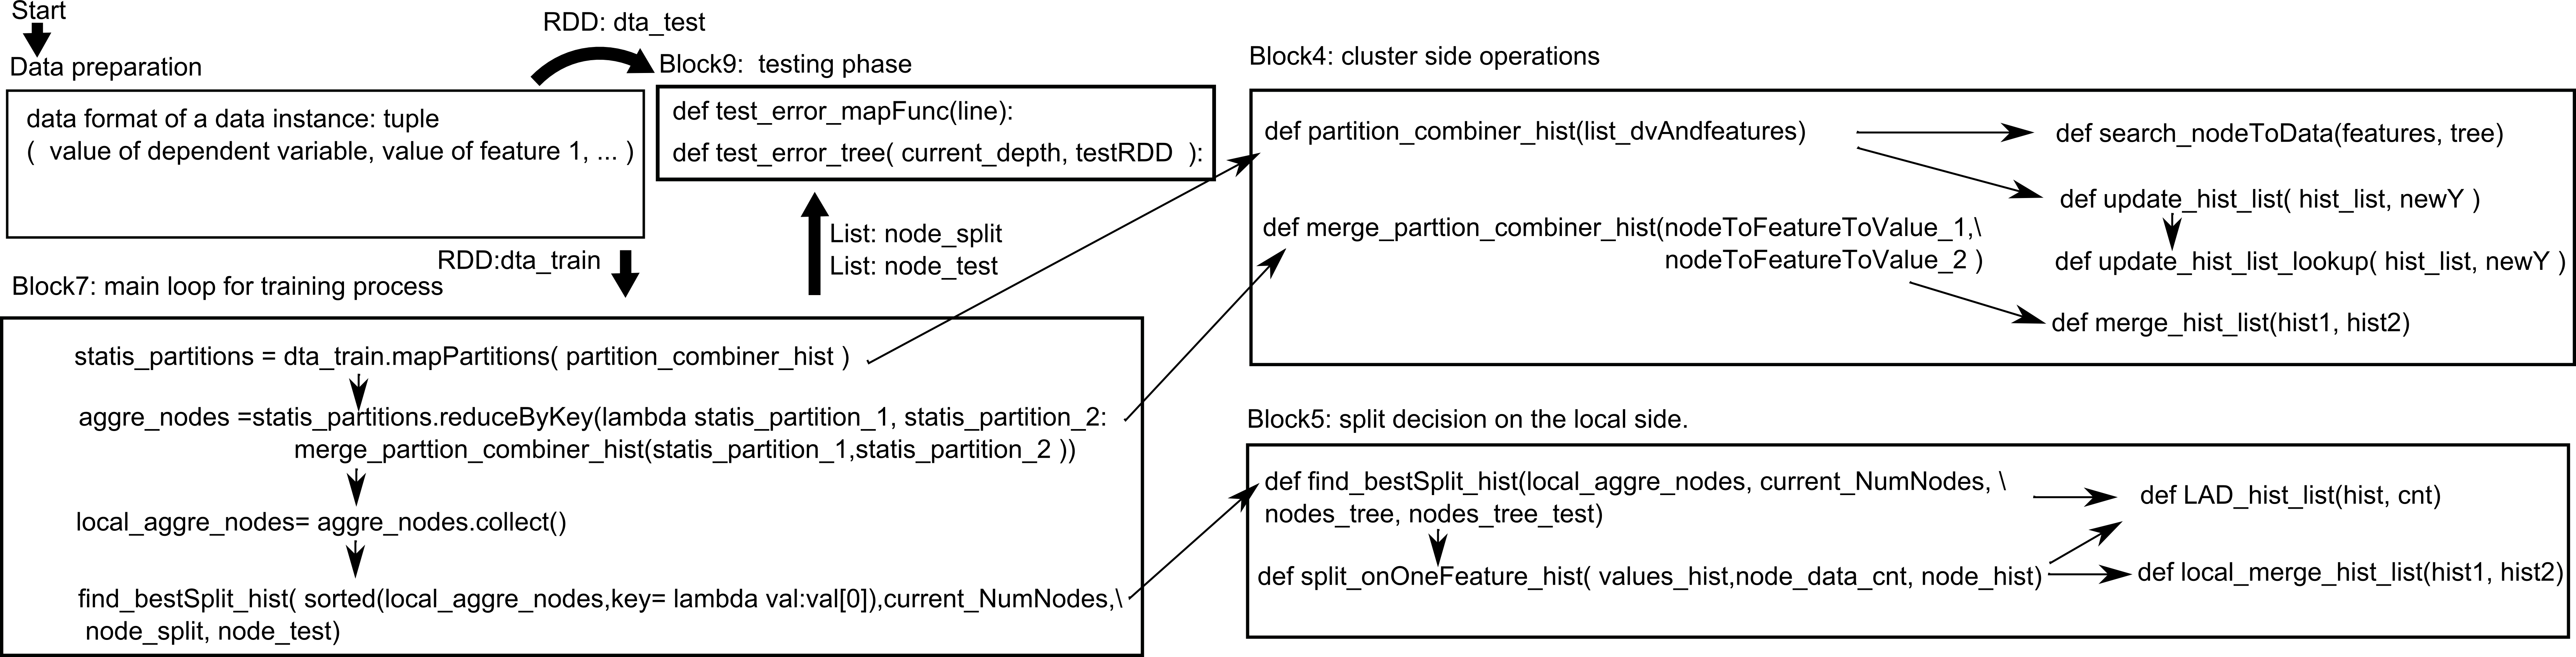
\includegraphics[width=1.95\columnwidth]{fig/design/block} 
%    \vspace{-0.2cm}	
    \caption{Function diagram of the system}
   \label{fig:design}
\end{figure*}

\subsection{Instructions}

Refer Figure \ref{fig:design} for illustrations.

\textbf{Step1: Data preparation} A data instance in the training and
testing datasets should be of the form $[$ value of dependent variable, value of feature 1, value of feature 2, $\ldots, ]$.

Note that our current approach focuses on categorical features. Feature values must be integers.
Moreover, it is recommended to reset feature values for efficiency issue, which means to
reset the feature values of raw dataset by the indexes of the values. For instance, if a feature has discrete values
such as $[1,200,300]$, it is better to reset them as $[1,2,3]$ by using a mapping $[1 \rightarrow 1, 200 \rightarrow 2, 300 \rightarrow 3]$.
 

\textbf{Step2: Block7 main loop for training process}
Sample from the whole dataset to obtain the training and testing datasets.
Call function $mapPartitions()$ of training data RDD to perform the data partition based histogram construction,
which is realized by functions in \textit{Block4 cluster side operations}.

Then, call function $reduceByKey()$ to merge the histograms over different data partitions on the cluster
to obtain unified histograms for each feature-value of each tree node. Now you can collect it from the cluster 
to a local place, where the split decision procedure is performed later.

Function $find\_bestSplit\_hist()$ on the local node calls functions in \textit{Block5 split decision on the local side}
to find the best splits for tree nodes layer by layer. 

\textbf{Step3: Block9 testing phase}
Testing phase is performed in a depth-increasing way to investigate the varying of test errors.
Starting from a regression tree with depth $2$, testing phase increases the depth one by one
and gets the testing error on each depth on the testing dataset.

Variables $node\_split$ and $node\_test$ contain the split and estimation information for each tree node.
Testing phase utilizes them to locate the tree node which a testing data instance belongs to and the value estimation on 
that tree node. Then, MSE over the testing data set is calculated.  


\noindent\textbf{Running example}

\textbf{Step1:} Load a previously generated synthetic data from the local file system. 
Block2 will automatically reset the feature values.

\textbf{Step2:} Compile block4, block5.

\textbf{Step3:} Sample training and testing datasets from the whole dataset
by setting the sample ratio in function 

$dta.cache().sample(False, \mathbf{.3}, 12345)$ 

\textbf{Step4:} Set the training parameters in block7

\begin{itemize}
\item $maxdepth$: maximum depth of regression tree to train.

\item $numFeatures$: number of features in the dataset.

\item $bin\_num$: limit on the number of bins in histograms.
\end{itemize}

Now run block7.

\textbf{Step5:} run block8 to store data for the following evaluation.

\textbf{Setp6:} run block9 to test the regression tree. 

